\chapter{Introdução}
\graphicspath{{chapter-01/img-cap01/}}

A extensão de alcance em projéteis é um tema de grande interesse para pesquisas sobre aerodinâmica. Isto se deve ao fato de que estes corpos são lançados a altas velocidades, portanto é necessário entender as forças atuantes a cada disparo. Para aumentar o deslocamento do corpo, procura-se reduzir o arrasto aerodinâmico, tendo em vista que é a principal força atuante em escoamentos viscosos. A \autoref{fig1:redarrasto} traz um resumo acerca das possibilidades em reduzir esse efeito no deslocamento, como \citeauthor{Dali2018a} demonstrou em seus estudos.

\begin{figure}[!ht]
	\centering
	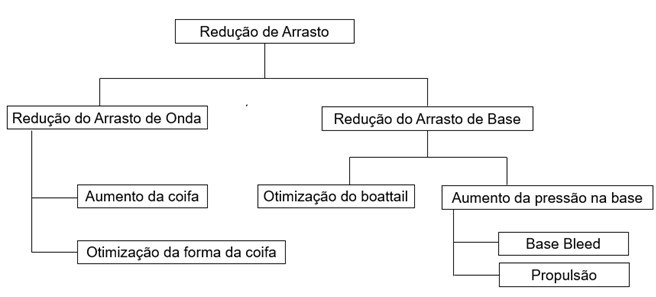
\includegraphics[width=1.0\textwidth]{foto01-reducao-arrasto.png}
	\caption[Técnicas de redução de arrasto, traduzido e adaptado.]{Técnicas de redução de arrasto \cite{Dali2018a}.}
	\label{fig1:redarrasto}
\end{figure}

Para os projetis, o arrasto se divide em três grandes grupos: o arrasto de pressão (excluindo a base), o arrasto viscoso e o arrasto de base. \citeauthor{Sahu1985} argumenta que em regime transônico, o arrasto de base pode compreender \qty{50}{\percent} da magnitude da força de resistência do ar. Como a própria Figura \ref{fig1:redarrasto} indica, pode-se modificar a forma do \textit{boattail} ou fazer uso de uma tecnologia que aumente a pressão na base do projetil. \citeauthor{Sedney1966} apresentou em seu trabalho que modificar o \textit{boattail} pode ser uma saída complexa, pois há a possibilidade de incrementar a expansão de Prandtl-Meyer, dificultando a medição do arrasto total presente.

Com esta informação, o foco deste trabalho é estudar a influência do escoamento existente na base do armamento com alcance estendido (ER), já que há muitos desafios para o desenvolvimento destes produtos. A granada a ser estudada possui calibre \qty{155}{\millimetre} (vide \autoref{fig2:cad-155mm}), devido à sua larga aplicação militar. O perfil axissimétrico possui características de design similares ao estudo feito por \citeauthor{Mahmoud2009}.

\begin{figure}[!ht]
	\centering
	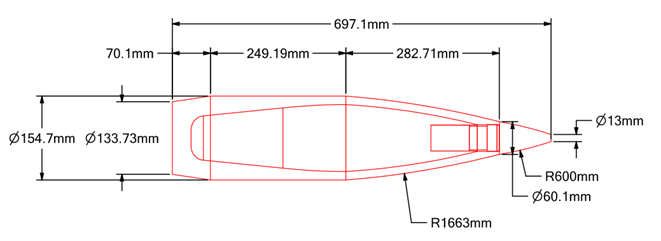
\includegraphics[width=1.0\textwidth]{foto02-cad-155mm.png}
	\caption[Granada hipotética de calibre \qty{155}{\millimetre} M107 HE.]{Granada hipotética de calibre \qty{155}{\millimetre} M107 HE.}
	\label{fig2:cad-155mm}
\end{figure}

Apesar de sua geometria relativamente simples, há necessidade de analisar como a injeção de massa de gases em altas temperaturas contribuem para a mudança do escoamento na base do projétil de tal forma que reduzam o arrasto ali presente. A tecnologia que aplica esses gases a partir da combustão de propelentes químicos se chama \textit{Base Bleed} (BB). A \autoref{fig3:esquemabb} apresenta como o escoamento percorre na região de maior interesse para o projeto.

\begin{figure}[!ht]
	\centering
	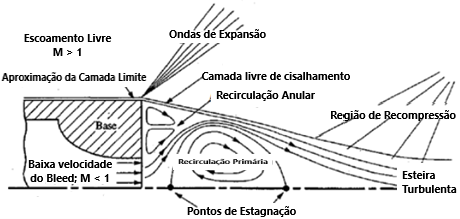
\includegraphics[width=0.8\textwidth]{foto03-esquema-bb.png}
	\caption[Escoamento supersônico na base de um projetil com \textit{Base Bleed}.]{Escoamento supersônico na base de um projetil com \textit{Base Bleed} \cite{Mathur&Dutton1996}.}
	\label{fig3:esquemabb}
\end{figure}

Para analisar qualitativamente o desempenho da tecnologia BB, o parâmetro adimensional de injeção, \(Inj\), foi definido como a razão entre taxa de vazão mássica dos gases e o produto do fluxo de massa do ar livre pela área da base do projetil. Atender valores ideais deste número adimensional é um grande desafio em desenvolver um projetil com \textit{Base Bleed}. \citeauthor{Andersson1976} demonstra a importância deste controle, pois o fluxo de massa deve ser um valor muito pequeno, conforme a \autoref{fig4:andersson1976} abaixo.

\begin{figure}[!ht]
	\centering
	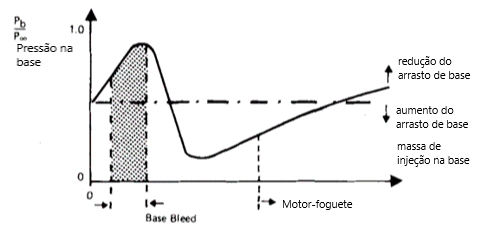
\includegraphics[width=0.8\textwidth]{foto04-grafico-andersson1976.png}
	\caption[Pressão na base por fluxo de massa.]{Pressão na base por fluxo de massa \cite{Andersson1976}.}
	\label{fig4:andersson1976}
\end{figure}

Segundo \citeauthor{Jelic2016Aug}, a existência do fenômeno de redução do arrasto de base através de um gerador de gás é datada desde a Segunda Guerra Mundial, quando se fazia uso de mísseis balísticos com traçadores que retardavam a redução de velocidade de voo, prolongando o alcance. Contudo, somente após a década de 1960 é que começou a se desenvolver pesquisas mais profundas, sendo o hidrogênio \(H_2\) o principal material usado nos geradores por ter baixo peso molecular e operar em altas temperaturas.

Os grandes questionamentos acerca deste combustível é que, apesar de muito eficiente, se permitia muito pouca estocagem dentro das munições e diminuía a vida útil delas. Outro fator relevante é que o gerador deveria conter muitos componentes, dificultando a manutenção. A solução encontrada foi trabalhar com propulsão sólida, já que se faz uso de muito menos equipamentos e o propelente poderia ser produzido através de compósitos com características adequadas às necessidades do projeto.

Segundo \citeauthor{Mahmoud2009}, para poder predizer as forças e momentos presentes na trajetória do projétil, existem quatro técnicas: os métodos empíricos; os testes em túneis de vento; simulação de fluidodinâmica computacional; e teste \textit{spark range}. As simulações recorrem métodos numéricos de fluidodinâmica computacional (CFD). Em razão das altas velocidades de disparo e das condições ambientais, considera-se o escoamento como compressível e turbulento, o que influencia nas equações de governo (Navier-Stokes) e de estado, assumindo que o ar do meio externo seja tratado como um gás perfeito. Em se tratando de turbulência, pretende-se verificar quais técnicas de abordagem sobre as equações de governo oferecem resultados satisfatórios a menor custo computacional. Em primeira análise, o objetivo é predizer os coeficientes aerodinâmicos sem a influência do \textit{Base Bleed} sob o ângulo de ataque (AOA) igual a zero.

Ao final deste trabalho é esperado concluir se a injeção de propelentes em combustão na base do projetil é um método eficiente para redução de arrasto. Para tal conclusão, será necessário validar os resultados das simulações CFD com o modelo de trajetória, como apresentado por \citeauthor{Rosendo2020}, atestando a influência da vazão e da temperatura dos gases injetados a montante do projetil. Em razão do projetil ser perfeitamente axissimétrico, a predição de trajetória é feita a partir do modelo ponto-massa modificado (MPMTM), desenvolvido por \citeauthor{Lieske1966} e padronizado pela OTAN através de um acordo de padronização chamado STANAG 4355 \cite{stanag4355}. 

Para assegurar a eficácia do programa desenvolvido, uma comparação com o PRODAS®, programa comercial para cálculos de dinâmica de voo para mísseis e foguetes, foi realizada considerando vários ângulos de elevação (QE) do tiro. Após a ratificação do código foram implementado os resultados do CFD para coeficiente de arrasto, seja a munição com ou sem \textit{Base Bleed}. 

\section{Revisão Bibliográfica}

O estudo sobre projéteis com alcance estendido (ER) que utilizam \textit{Base Bleed} começaram por meio de estudos experimentais que pretendiam verificar formas de reduzir o arrasto de base. \citeauthor{Sedney1966} e \citeauthor{Andersson1976} revelaram em seus trabalhos os testes realizados, sejam por testes de tiro ou em túneis de vento, com o objetivo de verificar a influência das forças de translação ou de rotação, além de verificar o efeito que o movimento rotacional causava no processo de combustão.

\begin{figure}[!ht]
	\centering
    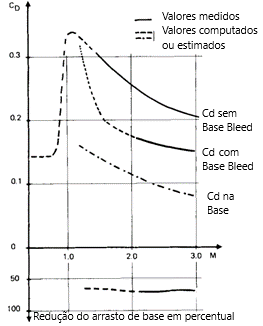
\includegraphics[width=0.6\textwidth]{foto05-grafico2-andersson1976.png}
	\caption[Coeficiente de Arrasto em função do número de Mach para um projétil calibre 120mm obtido por testes de tiro, com ou sem \textit{Base Bleed}.]{Coeficiente de Arrasto em função do número de Mach para um projétil calibre 120mm obtido por testes de tiro, com ou sem \textit{Base Bleed} \cite{Andersson1976}}
	\label{fig5:andersson1976}
\end{figure}

\citeauthor{Lieske1966} explica que o modelo MPMTM é o método principal de preparação de tabelas de tiro, desde que se saiba as propriedades de massa do projetil; os coeficientes aerodinâmicos e os valores experimentais dos testes de alcance. Para aprimoramento do trabalho, o projetil \qty{155}{\millimetre} M107 foi analisado, principalmente para ajustar o coeficiente da força Magnus para as simulações. A relevância deste trabalho recai até os dias atuais, tendo em vista que os países-membros da Organização do Tratado do Atlântico Norte (OTAN) fazem uso deste recurso para desenvolver projetis de longo alcance, sejam eles estabilizados por rotação ou por aletas \cite{stanag4355}.

\citeauthor{Sahu1985} apresentou uma proposta de analisar o escoamento na base do projetil a partir de simulações computacionais com métodos numéricos para resolução das equações de Navier-Stokes. As munições \qty{155}{\millimetre} foram analisadas a partir do regime transônico, pois segundo os autores, o arrasto de base representa \qty{50}{\percent} de todo o arrasto presente na dinâmica de voo. Neste trabalho, também é possível verificar a adição de massa de gás na base do projetil, o que demonstrou os efeitos do \textit{Base Bleed} de acordo com vários parâmetros de injeção. Por fim os resultados são comparados valores experimentais e recursos semiempíricos, seja para as granadas que possuem a tecnologia inserida ou não. A relevância deste trabalho é muito grande, pois serve como modelo de referência para todos os trabalhos com CFD que estudam arrasto de base em projéteis com alcance estendido por BB.

\citeauthor{Mathur&Dutton1996} manusearam velocímetros de laser Doppler para mensurar perfis de velocidade e turbulência na região próxima à esteira depois do corpo cilíndrico em escoamento com número de Mach (M) igual a \num{2,5}. Neste mesmo trabalho, estimaram valores ideais de injeção do fluxo de massa na base, ou seja, o ponto que oferece a maior pressão na base, onde a região primária de recirculação é mínima, assim como a esteira turbulenta. Esse adimensional também serve até hoje como referência para calcular o efeito \textit{Base Bleed} na trajetória. 

\citeauthor{Kauri1997} já lida com simulações computacionais desenvolvidas por códigos autorais em que se aplica o modelo de turbulência \(\kappa-\varepsilon\) para um escoamento supersônico (M = 1,2) a uma granada \qty{155}{\millimetre} com ângulo de ataque igual a \ang{5}. Este modelo foi escolhido porque havia o interesse em evitar problemas com as regiões dos pontos de estagnação. Neste trabalho, conclui-se que a aplicação do método baseado na vorticidade (VBPL) até oferece bons resultados para a hipótese de Boussinesq, a não ser que haja muita turbulência. 

\citeauthor{Sahu1997} resolveu numericamente as equações de Navier-Stokes de forma implícita usando dois modelos de turbulência: modelo algébrico para viscosidade turbulenta (Baldwin-Lomax) e o esquema de duas equações \(\kappa-\varepsilon\). O escoamento foi aplicado apenas na região da base e após o corpo do projetil a com M = 2,46 e ângulo de ataque nulo. Para verificar os resultados, dados experimentais em testes sob mesmas condições foram obtidos e usados. A conclusão que se chegou nesta pesquisa é que os melhores resultados foram apresentados com o modelo \(\kappa-\varepsilon\) para a região próxima à esteira turbulenta e prediz a pressão na base com maior precisão.

\citeauthor{Lee2006Sep} examinou diferentes perfis de orifícios para um corpo de revolução em escoamento livre a M = \num{2,47}. As seguintes considerações foram feitas para resolver as equações de Navier-Stokes com o modelo de turbulência \(\kappa-\omega\): perfil axissimétrico, escoamento compressível, com a média das massas, esquema totalmente implícito de volumes finitos e esquema \textit{upwind} de 2\textsuperscript{a} ordem para discretização espacial. A motivação inicial deste trabalho partiu do interesse em entender a redução do arrasto no regime supersônico, e verificar se estava de acordo com os resultados dos experimentos encontrados \cite{Bourdon2003Feb}.

Para averiguar a qualidade da simulação em CFD, o escoamento na saída do \textit{Base Bleed} foi calculado a partir das relações isentrópicas. O perfil da munição estudado concentrou somente a região da base, como mostra a Figura 6. Adotando um programa comercial, foi possível gerar uma malha computacional que garantiu as condições de contorno e melhor convergência. As regiões com maior gradiente de pressão concentraram maior quantidade de elementos. Ao todo, \num{50000} elementos foram suficientes para adquirir soluções com este domínio.

\begin{figure}[!ht]
	\centering
	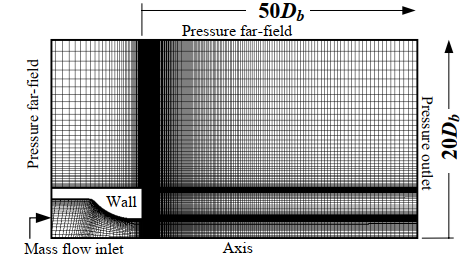
\includegraphics[width=0.6\textwidth]{foto06-malha-lee&kim.png}
	\caption[Malha computacional]{Malha computacional \cite{Lee2006Sep}}
	\label{fig6:lee2006}
\end{figure}
	
O escoamento na base pode ser visto na Figura \ref{fig7:bourdon2003} a partir dos resultados experimentais \cite{Bourdon2003Feb}. As imagens foram conseguidas utilizando a técnica de fluorescência planar em laser induzido (PLIF), que são mais profundamente detalhadas na referência. Já na \autoref{fig8:lee2006}, \citeauthor{Lee2006Sep} reproduziu computacionalmente as recirculações mais presentes próximas à base e ao eixo de simetria. Conforme I aumenta, a região primário de recirculação (PRR) é praticamente nula, embora haja a formação de uma nova recirculação próximo à camada de formação da esteira turbulenta. A conclusão confirma que há um valor adimensional que varia a cada projetil e suas condições de voo que maximiza a pressão na base. Uma configuração de design com maior área do orifício de saída dos gases ofereceu melhor controle na redução do arrasto, enquanto os casos em que a área de saída dos gases era muito pequena o incremento de injeção de massa resultou no efeito adverso na diminuição do arrasto de base. 

A influência do trabalho de \citeauthor{Lee2006Sep} é vista nas referências para as simulações em CFD sobre o arrasto de base, cujo modelo de turbulência \(\kappa-\omega\) é abordado em muitos estudos devido às limitações do sistema \(\kappa-\varepsilon\) em analisar a região próxima à parede. A abordagem sobre a independência de malha é percebida através dos resultados sobre o perfil de velocidades em função do raio do projetil. As condições de contorno serviram como parâmetros norteadores para aplicação na proposta da dissertação.

\begin{figure}[!ht]
	\centering
	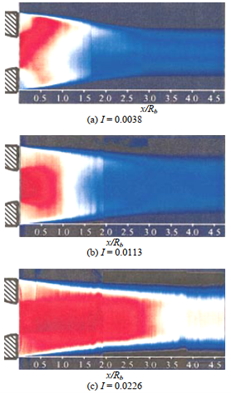
\includegraphics[width=0.5\textwidth]{foto07-bourdon2003.png}
	\caption[Visualização experimental]{Visualização experimental \cite{Bourdon2003Feb}}
	\label{fig7:bourdon2003}
\end{figure}

\begin{figure}[!ht]
	\centering
	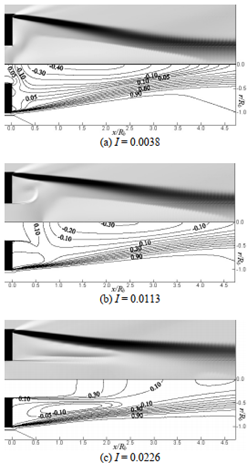
\includegraphics[width=0.5\textwidth]{foto08-base-lee&kim.png}
	\caption[Imagens computacionais baseadas no gradiente de densidade e contornos de velocidade adimensional em função do fluxo de ar no meio externo.]{Imagens computacionais baseadas no gradiente de densidade e contornos de velocidade adimensional em função do fluxo de ar no meio externo. \cite{Lee2006Sep}}
	\label{fig8:lee2006}
\end{figure}

\citeauthor{Mahmoud2009} analisou três perfis diferentes para investigar as propriedades do escoamento no entorno da munição em diferentes números de Mach com ângulo de ataque zero. Os três casos foram: com \textit{boattail}, com cavidade na base e com \textit{Base Bleed}. Além do mais, combinações entre eles foram investigadas. A maior redução de arrasto de base foi verificada quando se alinhava as três técnicas juntas. Para este caso, foi constatado uma redução de \qty{60}{\percent} do coeficiente de arrasto em regime subsônico e algo de \qtyrange{20}{30}{\percent} para os regimes transônico e supersônico. 
	
Ainda se tratando do trabalho de \citeauthor{Mahmoud2009}, percebe-se um detalhamento acerca dos fatores que afetam o arrasto na base do projetil, além do esclarecimento sobre o tratamento da malha em seu domínio, que pode ser visto na \autoref{fig9:mahmoud2009}. Por fim, o modelo RANS (\textit{Reynolds-Averaged Navier-Stokes}) atribuído a esta referência é o Spalart-Allmaras, cujas principais aplicações envolvem pesquisas sobre aerodinâmica.  

\begin{figure}[!ht]
	\centering
	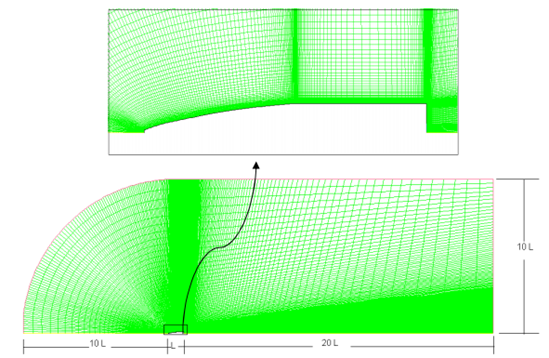
\includegraphics[width=1.0\textwidth]{foto09-malha-mahmoud2009.png}
	\caption[Modelo computacional para um projétil \qty{155}{\millimetre}.]{Modelo computacional para um projétil \qty{155}{\millimetre}. \cite{Mahmoud2009}}
	\label{fig9:mahmoud2009}
\end{figure}

\citeauthor{torangatti2basawaraj} concentrou as análises nas comparações entre as simulações computacionais por volumes finitos (CFD) e as abordagens semiempíricas para obtenção do arrasto, tais como MCDRAG, NSWCAP e Aero-Prediction. O modelo de turbulência RANS utilizado neste trabalho foi o \(\kappa-\varepsilon\). Ao contrário da maioria dos estudos sobre CFD para problemas relacionados a este, foi usado o esquema explícito de resolução do caso. A malha computacional desenvolvida utilizando programas comerciais apresentou uma forma de criar uma região com elementos estruturados.
	
\citeauthor{Sor2012Nov} faz um estudo similar ao anterior \cite{torangatti2basawaraj}, embora haja um aprofundamento maior acerca dos efeitos de compressibilidade e das teorias as forças aerodinâmicas. Em relação ao CFD, comparou-se os coeficientes de sustentação e de arrasto com possíveis ângulos de ataque, exceto os efeitos relacionados à rotação do projetil no disparo.

Para aprimorar o modelo com 4 graus de liberdade (4-DOF) que é desenvolvido para descrever a trajetória do projetil, estudos mais recentes foram realizados para mitigar as limitações existentes da STANAG 4355 \cite{Baranowski2013-1,Baranowski2013-2,Baranowski2013-3}. Para isso, foi necessário comparar o modelo 4-DOF com o clássico modelo de corpo rígido de 6 graus de liberdade (6-DOF) a partir de 5 ângulos de elevação para ajustar os fatores de forma, tal como descreve a STANAG 4144. O grande benefício do MPMTM é prover resultados ao menor custo computacional possível, o que significa menor tempo para resolver um problema durante uma guerra, onde este fator é crítico \cite{Baranowski2013-2}.

\citeauthor{Jelic2016Aug} teve como principal objetivo investigar vários métodos de incremento de alcance e propor soluções ótimas para estender alcance de sistemas de artilharia existentes. Dentre todas as metodologias para estender o alcance, o foco do trabalho foi pesquisar sobre \textit{Base Bleed} e motores com propulsão sólida (SRM). A pesquisa envolveu cálculos teóricos, simulações numéricas e validação através de experimentos, com resultados que confirmaram a viabilidade do conceito. 
	
\citeauthor{Xue2016Oct} desenvolveu simulações numéricas para investigar o arrasto de base e os efeitos causados pela injeção do gases pós-combustão em regime supersônico. Modelos químicos detalhados de combustão de \(H_{2}-CO\) foram incorporados dentro do código computacional produzido em FORTRAN com as equações de Navier-Stokes com a aplicação do modelo RANS SST \(\kappa-\omega\) \cite{Menter1994TwoequationET}. Por fim, os resultados foram validados a partir de dados experimentais e providenciaram uma melhor compreensão dos benefícios de utilizar a tecnologia \textit{Base Bleed}. O ponto alto deste estudo é permitir aplicar os efeitos da combustão dentro da pesquisa sobre a aerodinâmica do projetil. 
	
\citeauthor{belaidouni2016} estudou um armamento de calibre \qty{122}{\millimetre} com perfil axissimétrico resolvendo numericamente as equações de governo para os regimes transônico e supersônico com dois modelos diferentes de turbulência por meio de volumes finitos. Ambos os resultados foram comparados com dados de predições semiempíricas para os coeficientes aerodinâmicos. Ao contrário dos outros trabalhos, apostou-se numa malha tridimensional para o domínio do trabalho. No desenvolvimento deste projeto a injeção de massa é calculada através das equações correspondentes para a balística interna que serviram aos testes estáticos da geradora de gás. Considerando ângulo de ataque nulo, verificou-se a redução de \qty{12}{\percent} do arrasto gerado na base da munição. A escolha final do autor pelo modelo de turbulência foi o \(\kappa-\varepsilon\) realizável.
	
\citeauthor{nicolas-perez_accuracy_2017} tratou de abordar diferentes modelos RANS, DES (\textit{Detached eddy Simulation}) e LES (\textit{Large-eddy Simulation}) para estimar o coeficiente de arrasto de corpos delgados com rotação e \textit{Base Bleed} sob regimes transônico e supersônico quasi-permanentes (número de Mach entre \numlist{0,9;1,5}). Diferentes malhas foram testadas, além de simular condições com ou sem injeção de massa gasosa na base do projetil, como na Figura \ref{fig10:nicolas2017}. Uma observação relevante neste trabalho é do esquema de fluxo ROE-FDS, pois se afirma que este recurso oferece bons resultados em casos com escoamento compressível.

\begin{figure}[!ht]
	\centering
    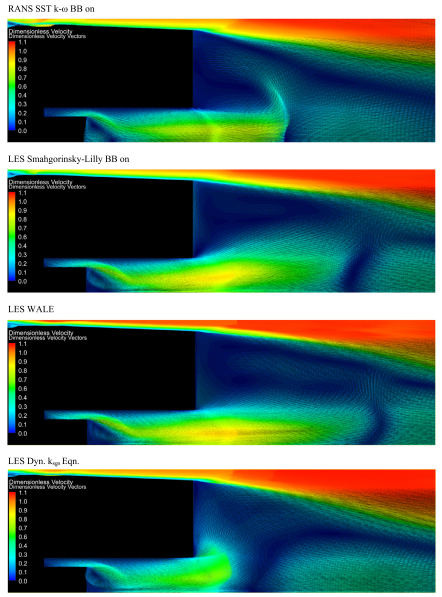
\includegraphics[width=0.5\textwidth]{chapter-01/img-cap01/foto10-nicolas2017}
	\caption[Campo de velocidade com M = \num{1,5} em diferentes modelos de turbulência.]{Campo de velocidade com M = \num{1,5} em diferentes modelos de turbulência. \cite{nicolas-perez_accuracy_2017}}
	\label{fig10:nicolas2017}
\end{figure}

A constatação sobre os resultados foi de que as abordagens RANS e DES obtiveram baixa acurácia em predizer o arrasto quando encararam o problema envolvendo uma camada de gases misturados em alta temperatura com a esteira transônica, ou seja, dificuldade em analisar a eficiência da geradora de gás. Quando inativo, os dois modelos recém citados ofereceram dados relevantes, se comparados aos valores de referência para o projeto em questão. Por fim, acrescentou o fato de que a temperatura dos gases injetados foi muito mais influente do que o peso molecular deles. Dentre os modelos de turbulência aplicados, o que melhor se adaptou aos resultados experimentais foi o caso LES WALE (\textit{Wall Adapting Local Eddy}) \cite{nicolas-perez_accuracy_2017}.

\citeauthor{Dali2018a} utilizou simulações CFD para analisar propriedades do arrasto de base em projetis com BB. Mais de um tipo de grão propelente foi usado. A meta era encontrar um caminho para efetivamente controlar o fluxo na base para reduzir o arrasto na região e otimizar utilizando um programa adequado para tal. Os modelos de turbulências aplicados foram o SST \(\kappa-\omega\), transição \(\kappa-\kappa l-\omega\) e modelo de tensão de Reynolds (RSM). As propriedades da vazão mássica foram adimensionalizadas para melhor compreensão dos resultados. Para cada grão propelente, observou-se um parâmetro ótimo de injeção e depende da temperatura dos produtos da combustão. Em valores concretos, o arrasto reduziu em torno de \qty{7}{\percent} para o \textit{Base Bleed} a \qty{300}{\kelvin} e mais de \qty{28}{\percent} para os gases ejetados a \qty{2500}{\kelvin}. Este estudo também reafirmou a irrelevância do peso molecular dos produtos da combustão na redução do arrasto.
	
\citeauthor{Dali2018b}, por meio de um programa proprietário CFD, analisou as duas principais formas de redução de arrasto na base de uma munição \qty{122}{\millimetre}. Primeiro, a área de concentração esteve na otimização da estrutura do \textit{boattail}. Em seguida, pesquisou a influência de alterar a pressão na base do projetil com \textit{Base Bleed}, inclusive com variações de ângulos de saída dos gases em relação ao eixo longitudinal da granada. Comparando os valores obtidos com as referências encontradas em predições semiempíricas, as diferenças foram quase imperceptíveis. Acerca da verificação com dados de radares 3D, a hipótese mais viável é do nível de ruído dos sinais, que dificultam as medidas de velocidade durante o voo. O trabalho serviu como uma referência introdutória ao assunto discutido na proposta da dissertação e oferece outras possibilidades de estudo sobre a otimização da aerodinâmica de perfis balísticos. 
	
Há trabalhos no Brasil acerca do mesmo tema, como \cite{Lucena2020,Rosendo2020,Gil2020}, que exploraram uma abordagem semelhante a esta pesquisa, contudo enfatizando a munição \qty{114}{\millimetre} desenvolvida pela EMGEPRON, uma empresa estatal ligada à Marinha do Brasil. Na questão da simulação de fluidodinâmica computacional, o foco foi num domínio bidimensional e axissimétrico, com a malha não estruturada, além de não aplicar nenhum modelo de turbulência para resolver o escoamento. O OpenFOAM®, um programa \textit{open-source}, foi escolhido para resolver o caso, onde se desenvolveu um modelo viável para predizer uma específica formulação para um propelente a ser utilizado em munições com alcance estendido, tendo em vista que não havia no mercado programas comerciais para entregar tal serviço. 

O único caminho que a Marinha do Brasil até então encontrava era a partir de lançamentos balísticos de granadas como teste, o que era caro e com alto risco de segurança. Logo, através de um domínio bidimensional e axissimétrico, as equações de governo para um escoamento supersônico de uma granada calibre \qty{114}{\millimetre} foram resolvidas. A conclusão desta pesquisa é que a velocidade e a temperatura de injeção dos gases do \textit{Base Bleed} possuem um valor ideal para reduzir o arrasto.

\citeauthor{Reddy2021} apresentou simulações numéricas sobre projetis de calibre \qty{155}{\millimetre}, seja com ou sem \textit{Base Bleed}, em regime supersônico (M = \num{2,26}). Para tal trabalho, todo o desenvolvimento foi realizado de uma ferramenta comercial. O algoritmo aplica o modelo de turbulência SST \(\kappa-\omega\), variando o ângulo de ataque entre \qtylist{0;10}{\degree}. Usando os recursos experimentais, as simulações foram comparadas e observou-se uma redução do coeficiente de arrasto na ordem de 14\% ao considerar o efeito \textit{Base Bleed}. 

\section{Motivação}

A dinâmica dos fluidos computacional trata-se de uma área da engenharia que vem crescendo ao longo dos últimos anos, com o avanço tecnológico. Existem inúmeros casos na natureza e na engenharia de escoamentos turbulentos com separação de fluxo que merecem ser estudados, que podem ser aprofundados e facilitados através de simulações numéricas computacionais. Nos problemas aerobalísticos, a redução de arrasto é objeto de estudo de muitas pesquisas, pois cria oportunidades em atuar na fronteira do conhecimento sobre desempenho de corpos balísticos, sejam projéteis, mísseis ou foguetes. A utilização da tecnologia \textit{Base Bleed} se apresenta como um desses casos porque permite a fabricação de equipamentos com um princípio de funcionamento relativamente simples, contudo há um desafio em matéria de design do produto e da dinâmica de fluidos existente na base do armamento.

Ao longo das últimas décadas os estudos sobre redução de arrasto na base manejando simulações numéricas computacionais tornaram-se mais frequentes. Primeiramente a abordagem CFD permitiu diminuição de testes experimentais para validação dos produtos, tendo em vista que os testes de tiro são dispendiosos, ainda mais quando se adota diferentes configurações de granadas para o disparo (com ou sem BB; com ou sem \textit{boattail}, fora os diferentes formatos). Após esses fatos, este projeto pretende aumentar a cadeia de pesquisas relacionadas com este tema no Brasil, além dos já estabelecidos \cite{Lucena2020, Rosendo2020, Gil2020}. Inclui-se ao fato de que no mercado não há modelos ou mesmo serviços que permitam estudar os efeitos da combustão do \textit{Base Bleed} de acordo com a composição química de seus propelentes. 
	
Os fenômenos de turbulência presentes no escoamento no entorno do projetil, sobretudo à jusante de sua base, serão estudados e analisados com duas abordagens RANS para descrever a turbulência do ar, principal fluido de escoamento da granada. Ao escolher os modelos RANS, espera-se obter resultados com maior agilidade e razoável confiabilidade, motivo que é amplamente mais usado na indústria ao ser comparado com modelos DES, LES ou DNS. Todavia, há de se olhar para os valores de referência ou de dados experimentais, se houver. Incorpora-se os resultados obtidos com os códigos desenvolvidos para a predição de trajetória para ofertar uma solução mais acessível se comparado ao PRODAS®, principal referência do setor aeroespacial para resolução deste tipo de problema.

Sendo assim, o presente trabalho contribuirá para a comunidade da dinâmica dos fluidos computacional tanto em relação ao estudo de metodologias para redução de arrasto na base em perfis aerodinâmicos quanto para o estudo da formulação da geradora de gás e os possíveis propelentes a serem utilizados. Há também uma contribuição para o estudo de dinâmica de corpos rígidos para oferecer soluções mais fidedignas e práticas para aplicações das normas técnicas que envolvem as tecnologias militares, como ocorrem ao fazer uso dos acordos de padronização (STANAG) para produção de armamentos com respostas mais ágeis em situações reais de combate. Com o avanço da tecnologia computacional, a mitigação dos riscos associados aos materiais aplicados à produção do BB está cada vez maior. 

\section{Objetivo de Estudo}

O presente trabalho tem como objetivo o estudo sobre a aerodinâmica de um projetil de calibre \qty{155}{\millimetre}, principalmente sobre a influência da força de arrasto durante a trajetória balística. Nesta granada, será verificado o comportamento do arrasto total e na região da base, comparando os casos inerte (sem \textit{Base Bleed}) e o ativo (com \textit{Base Bleed}). Alguns parâmetros serão modificados para descobrir a melhor configuração possível do sistema BB, ou seja, qual situação que permite a maior redução do arrasto e como isso influencia a trajetória.
	
Em se tratando da fluidodinâmica computacional, as equações de governo consideram as seguintes propriedades: compressível, pois o regime de velocidades \(\left(\num{0,4} \leq M \leq \num{3,0}\right)\) apresenta variações na densidade do fluido do meio externo; permanente, logo as propriedades do fluido não variam em função do tempo; axissimétrico, porque o projetil possui um formato perfeitamente simétrico ao longo de um único eixo, o que é vantajoso para a análise CFD, pois essa aproximação é considerada uma técnica poderosa para reduzir o custo computacional \cite{Lucena2020}. Enquanto isso, as equações de estado consideraram o ar como gás ideal, assim como o gás ejetado pelo \textit{Base Bleed} e, especialmente a viscosidade dinâmica do fluido, que aplicou a Lei de Sutherland como técnica para registrar as variações do fluido de acordo com o gradiente de temperatura.

Acerca dos modelos de turbulência, o presente trabalho utilizou duas abordagens RANS. O escoamento turbulento é caracterizado por ter um comportamento difusivo, tridimensional e transiente \cite{Rezende2009}. A turbulência pode sofrer flutuações nas quais é possível aproximar de um escoamento estacionário, desde que se considere um intervalo de tempo adequado para a análise \cite{Souza2011,SilveiraNeto2002}. Em geral, a turbulência envolve grandes escalas temporais e espaciais, o que exige alto esforço computacional para obter resultados com qualidade através de simulações DNS. Por essa razão, os modelos RANS são considerados as opções mais práticas para predição numérica e são as mais empregadas pela indústria.
	
Dentre os modelos RANS existentes, foram escolhidos o Spalart-Allmaras \cite{Spalart1992} e o SST \(\kappa-\omega\) (\textit{Shear-Stress Transport} \(\kappa-\omega\)) \cite{Menter1994TwoequationET,Menter2003,Menter2009}. Cada modelo possui vantagens e desvantagens a serem exploradas, principalmente em problemas aerodinâmicos. A modelagem que oferecer os resultados mais confiáveis terão seus valores acoplados ao simulador desenvolvido neste projeto, assim como os coeficientes extraídos do PRODAS® para predizer o voo da granada.

Para determinar a influência na dinâmica de voo do projetil, um código computacional foi desenvolvido em MATLAB® a partir de um trabalho de Iniciação à Pesquisa feito no Instituto Militar de Engenharia (IME) \cite{ThallyoENCIT2022,Thallyo2022} para comparar com o PRODAS®, fazendo uso das mesmas condições de entrada necessárias para calcular o trajeto com 4 graus de liberdade. Atingindo os objetivos, atesta-se que o programa autoral está dentro do que é estabelecido pela STANAG 4355. Entretanto, a validação inicial não considera o uso da tecnologia BB, portanto é de suma importância verificar a influência da injeção de gases na base do projetil em função do alcance e do apogeu da munição. 

\section{Organização do Trabalho}

O segundo capítulo descreve uma revisão bibliográfica sobre o fenômeno físico da compressibilidade e das equações de governo que regem o fluido. A seguir, o Capítulo \ref{cap:metodos-numericos} introduz os métodos numéricos e as possíveis abordagens de discretização para as equações de transporte, com ênfase no Método de Volumes Finitos (MVF). No Capítulo \ref{cap:turbulencia}, a turbulência é apresentada como tópico de grande interesse devido aos altos números de Reynolds presentes no escoamento em torno da munição \qty{155}{\millimetre}. Em especial, será tratado com mais afinco os modelos de turbulência baseados nas médias de Reynolds (RANS) e as condições necessárias para o fechamento do sistema de equações de transporte resultante. Com estes tópicos, é possível analisar e compreender os efeitos aerodinâmicos a partir das simulações CFD.

Os modelos RANS selecionados para analisar o escoamento, são Spalart-Allmaras \cite{Spalart1992} e SST \(\kappa-\omega\) \cite{Menter1994TwoequationET,Menter2003,Menter2009}. Para a análise de trajetória, bem como a teoria necessária para implementação do modelo ponto-material modificado \cite{stanag4355}, foi desenvolvido o Capítulo \ref{cap:trajetoria}. A descrição do estudo proposto, explicando detalhadamente as condições de contorno para as simulações CFD e os valores iniciais para a predição de voo da munição \qty{155}{\millimetre}, pode ser encontrada no Capítulo \ref{cap:estudo-proposto}.

O Capítulo \ref{cap:resultados} finalmente apresenta e analisa os resultados obtidos com a variação de três parâmetros: o diâmetro de saída, a vazão mássica e a temperatura do propelente expelido pelo sistema \textit{Base Bleed}, referente ao escoamento compressível a jusante do projetil. Eis os resultados das simulações CFD: os coeficientes de arrasto sem ângulo de ataque em função do número de Mach, \(C_{D_{0}}\); contornos de pressão e velocidade; as linhas de corrente para demonstrar a formação da recirculação anular e do deslocamento da região de recirculação primária dentro da esteira turbulenta. A partir destes resultados é que pôde-se aplicar as equações de movimento para a trajetória, segundo a STANAG 4355 \cite{stanag4355}. No fim deste capítulo são abordadas as validações necessárias para o programa próprio em MATLAB® \cite{ThallyoENCIT2022,Thallyo2022}, bem como os resultados obtidos de possíveis disparos da munição \qty{155}{\millimetre} nas condições das simulações de dinâmica dos fluidos computacional. 

A conclusão do trabalho encontra-se no Capítulo \ref{cap:conclusoes}, resumindo os pontos principais, e discutindo os principais problemas encontrados e recomendações para trabalhos futuros.